\documentclass[11pt, oneside]{article}   	% use "amsart" instead of "article" for AMSLaTeX format
\usepackage{geometry}                		% See geometry.pdf to learn the layout options. There are lots.
\geometry{letterpaper}                   		% ... or a4paper or a5paper or ... 
%\geometry{landscape}                		% Activate for for rotated page geometry
%\usepackage[parfill]{parskip}    		% Activate to begin paragraphs with an empty line rather than an indent
\usepackage{graphicx}				% Use pdf, png, jpg, or eps� with pdflatex; use eps in DVI mode
								% TeX will automatically convert eps --> pdf in pdflatex		
\usepackage{amssymb}
\usepackage{amsmath}
\usepackage{parskip}
\usepackage{color}
\usepackage{hyperref}

\title{The Wave Equation}
%\author{The Author}
%\section{}
%\subsection*{}
\date{}							% Activate to display a given date or no date

\graphicspath{{/Users/telliott_admin/Dropbox/Tex/png/}}
% \begin{center} 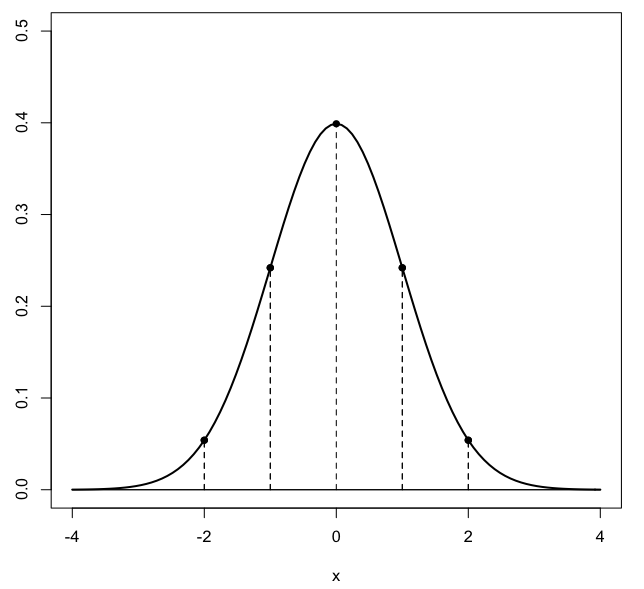
\includegraphics [scale=0.4] {gauss3.png} \end{center}
\begin{document}
\maketitle
\Large
This short write-up contains a derivation of the wave equation.  We consider a violin string pinned down at the ends and then plucked.  Here is a short segment of the string (the notation doesn't match exactly what I'm going to use, but it's a place to start).

\begin{center} 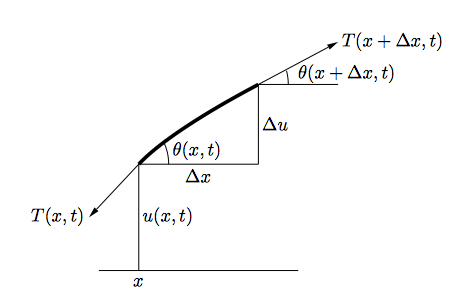
\includegraphics [scale=0.75] {wave1.png} \end{center}

Here, $x$ is not a variable but just a label for a position on the string.  We start to solve this problem by an approximation, saying that the tension $T$ (the force in the direction shown by the arrows), has the \emph{same magnitude} at both ends of the short interval shown as $\Delta x$ in the figure.  

What differs between the two ends of the interval and provides a net force is the difference in the angle $\theta$ at the two positions $x$ and $x + \Delta x$.  That force is
\[ T \sin \theta_{x + \Delta x} - T\sin \theta_x \]

which, by Newton's Law, is equal to $ma$.  For this small segment of the string

\[ T \sin \theta_{x + \Delta x} - T\sin \theta_x = dm \ a \]

where $dm$ is the mass of this small segment.  You might be tempted to write $\ddot{x}$ ($d^2 x/dt^2$) for $a$ here, but as we said, in this problem $x$ is just a label for a position on the string.

The value which changes is the displacement, which we will call $\psi$.  Furthermore, if you think about it, it is clear that the displacement $\psi$ is a function of both time and the horizontal coordinate $x$, so we need the partial derivative
\[ T \sin \theta_{x + \Delta x} - T\sin \theta_x = dm \ \frac{\partial^2 \psi}{\partial t^2} \]

Now, $dm$ is the mass of this small segment, which is equal to the mass per unit length times $dx$.
\[ T \sin \theta_{x + \Delta x} - T\sin \theta_x = \mu \ dx \ \frac{\partial^2 \psi}{\partial t^2} \]

On the left hand side we are going to apply the small angle approximation.  Recall that
\[ \sin \theta \approx \theta \]

(where the next term in the series for $\sin \theta$ is $-\theta^3/3!$).  Since $\cos \theta \approx 1$ then
\[ \theta \approx \sin \theta \approx \tan \theta \]

If you look back at the figure you will see that according to the labels there
\[ \frac{\Delta u}{\Delta x} = \tan \theta \]

Now, $u$ is what we are calling $\psi$ and in the limit as  this is really a partial derivative
\[ \frac{\partial \psi}{\partial x} = \tan \theta \approx \sin \theta \]

\[ T ( \frac{\partial \psi}{\partial x} \bigg |_{x + dx} - \frac{\partial \psi}{\partial x} \bigg |_{x})  =  \mu \ dx \ \frac{\partial^2 \psi}{\partial t^2} \]

Now, divide both sides by $T$ and by $dx$ and let $dx \rightarrow 0$ and we get

\[ \frac{\partial^2 \psi}{\partial x^2} =  \frac{\mu}{T}  \ \frac{\partial^2 \psi}{\partial t^2} \]
This is the wave equation, but we will re-write it as
\[ \frac{\partial^2 \psi}{\partial x^2} =  \frac{1}{v^2}  \ \frac{\partial^2 \psi}{\partial t^2} \]
\[ v = \sqrt{T/\mu} \]
It will turn out that $v$ is the velocity of the wave.

We just guess the solution
\[ \psi(x,t) = A \cos kx + \omega t \]
where $k$ is called the \emph{wave number}.

\[ \frac{\partial^2}{\partial x^2} \ \psi(x,t) = -k^2  \ \psi(x,t) \]
\[ \frac{\partial^2}{\partial t^2} \ \psi(x,t) = -\omega^2  \ \psi(x,t) \]

So 
\[ -k^2 = -\frac{ \omega^2}{v^2} \]
\[ k = \pm \frac{\omega}{v} \]
\[ \pm kv = \omega \]
\[ \psi(x,t) = A \cos kx - \omega t \]

At time zero, this function has a maximum at $x=0$.  Wait a time $dt$, then the maximum is when $k\ dx-\omega\ dt = 0$.
\[ \frac{dx}{dt} = \frac{\omega}{k} \]
Substituting $\omega = \pm kv$
\[ \frac{dx}{dt} = \pm v \]
and
\[ \psi(x,t) = A \cos kx \pm kvt = A \cos k(x \pm vt) \]
Clearly, the crest of the wave is moving at the velocity $v$.

\[ \psi(x,t) = A \cos k(x - vt) \]
describes a wave moving to the right, and the opposite choice of sign means a wave moving to the left.

Note that \emph{any} function $f(x - vt)$ satisfies the wave equation, even
\[ A e^{-k^2(x-vt)^2} \]

If $kx = 2 \pi$ the wave repeats and by definition
\[ k \lambda = 2 \pi \]
\[ k = \frac{2 \pi}{\lambda} \]

\[ v = \frac{\omega}{k} = \frac{\omega \lambda}{2 \pi} \]
since $\omega = 2 \pi f$
\[ v = f \lambda \]
The wavelength times the frequency is equal to the velocity.

\end{document}  